%
% Capítulo 1
%
\chapter{Introdução} \label{cap1}

A gestão de stocks é um processo estruturado, assim, no âmbito da \acrfull{iot} e de forma a simplificar o quotidiano de cada um, surge este projeto. Atualmente, são várias as aplicações responsáveis por fornecer listas de compras, porém carecem de controlo de stocks e conhecimento dos hábitos dos seus utilizadores. A aplicação desenvolvida neste projeto distingue-se pelo controlo de stocks existentes nos armários, frigoríficos e despensa. Difere-se também, pela presença de um algoritmo de previsão de stocks, com base no histórico de consumo e reposição do utilizador.

%
% Secção 1.1
%
\section{Enquadramento} \label{sec11}

No contexto do projeto assume-se a existência de duas formas de apresentação para os produtos: avulsos e embalados. Os primeiros são conservados em sistemas de arrumação marcados com \textit{tags} programáveis por \textit{smartphones}. Os detalhes dos itens são especificados pelo utilizador e carregados para a \textit{tag}. Enquanto que para os produtos embalados, admite-se que os produtores utilizam \textit{tags}, \acrfull{nfc} ou \acrfull{rfid}, para guardar os rótulos de forma digital e em formato standard.

Após a aquisição, os artigos são armazenados em locais que devem dispor de dispositivos de hardware equipados com leitores de \textit{tags}. É recolhida a informação presente na \textit{tag}, identificado o tipo de movimento (entrada ou saída) e enviado para a \gls{api-web}. 

\begin{figure}[H]
	\centering
	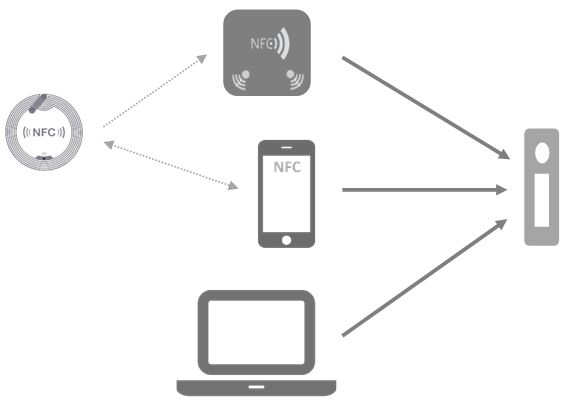
\includegraphics[width=13cm, scale=1]{./figures/project_structures.png}
	\caption{Estrutura do Projeto}
	\label{project-structure}
\end{figure}

\begin{center}
	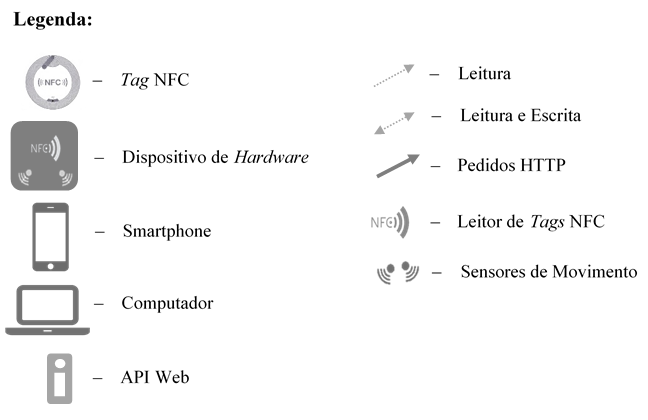
\includegraphics[width=12cm, scale=1]{./figures/project_structures_caption.png}
\end{center}

Com a Figura \ref{project-structure} pretende-se não só apresentar os principais componentes do projeto, bem como demonstrar de forma breve a relação dos mesmos. É de destacar que uma \textit{tag} tanto pode ser lida por um dispositivo de hardware munido de um leitor de \textit{tags}, como por um smartphone equipado com tecnologia \acrshort{nfc}. O mesmo smartphone pode ainda escrever na \textit{tag} \acrshort{nfc}, necessário para identificar produtos avulsos presentes num sistema de arrumação. Tanto o dispositivo de \textit{hardware} como as aplicações, móvel e \textit{web}, comunicam com a \gls{api-web}.

Através da aplicação disponibilizada, o utilizador poderá consultar:
\begin{itemize} \itemsep 0pt
	\item os produtos em stock,
	\item as listas do sistema e/ou as por si criadas,
	\item as suas casas e caraterísticas,
	\item as alergias dos membros de cada casa,
	\item os locais de armazenamento e dispositivos de hardware.
\end{itemize}

Será ainda possível:
\begin{itemize} \itemsep 0pt
	\item receber alertas de produtos perto do fim da validade,
	\item especificar stocks mínimos e/ou indesejados,
	\item partilhar listas entre utilizadores da mesma casa.
\end{itemize}

%
% Secção 1.2
%
\section{Metas e Objetivos} \label{sec12}
Têm-se como objetivos, os seguintes pontos:
\begin{itemize} \itemsep 0pt
	\item Desenho e Implementação das Aplicações Móvel e Web
	\item Desenvolvimento da \gls{api-web}
	\item Desenho e Implementação da \acrshort{db}
	\item Desenvolvimento do acesso à \acrshort{db}
	\item Aplicação da Lógica de Negócio no acesso à \acrshort{db}
	\item Elaboração do Algoritmo de Previsão de Stocks
	\item Realização dos Algoritmos necessários
\end{itemize}


%
% Secção 1.3
%
\section{Especificações do Projecto e Resumo da Solução} \label{sec13}

O projeto é composto por 2 blocos principais, que se relacionam. A Figura \ref{project-architecture} representa esses blocos. 

\begin{figure}[H]
	\centering
	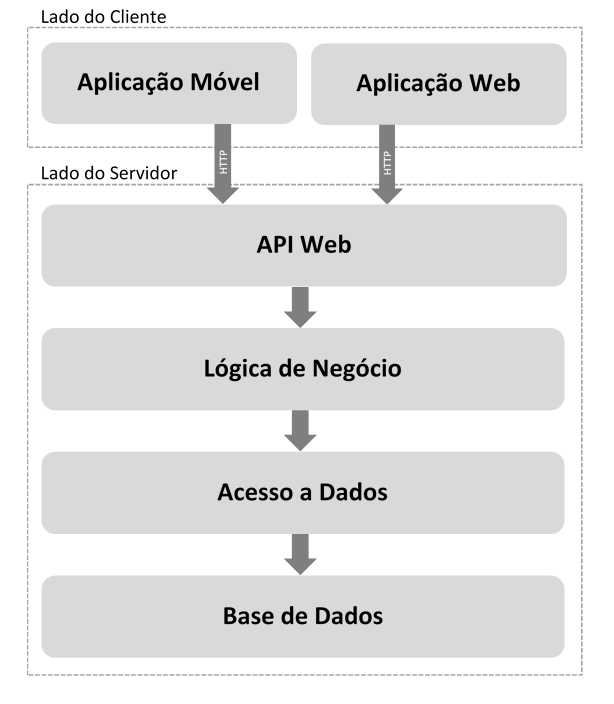
\includegraphics[height=10cm, scale=1]{./figures/project_architecture.png}
	\caption{Arquitetura do Projeto}
	\label{project-architecture}
\end{figure}

Um dos blocos é a interação com o utilizador, através de duas aplicações, uma móvel e uma Web. A aplicação móvel desenvolvida apenas para a plataforma \textit{Android}, e utilizando a linguagem \textit{Kotlin}. Para a aplicação Web, implementada recorrendo à linguagem \textit{JavaScript}, com o auxilio da \textit{framework Express}. 

O outro bloco incluí a \gls{api-web} desenvolvida com a \textit{framework} da \textit{Spring}, chamada de \textit{Spring Boot}. Subjacente a este última estão as camadas: \acrfull{db}, \acrfull{dal}, \acrfull{bll}.  A camada da base de dados (\acrshort{db}), realizada com o \acrfull{sgbd} \textit{PostgreSQL}. Para a camada de acesso a dados (\acrshort{dal}), responsável pelas leituras e escritas, a ferramenta utilizada é a linguagem de programação \textit{Java}, com a \gls{api} \acrfull{jdbc}. A camada da lógica de negócio (\acrshort{bll}), também se serve da ferramenta mencionada anterior para a sua implementação, esta camada é responsável pela gestão dos dados obtidos da \acrshort{db} ou da \gls{api-web}.


%
% Secção 1.4
%
\section{Estrutura do Relatório} \label{sec14}
O relatório está estruturado em 4 capítulos.

O capítulo 2 formula o problema, detalhando os requisitos do projeto. São ainda apresentadas as dificuldades encontradas ao longo do projeto. 

No capítulo 3 
